\chapter{Base Features}
\label{ch:base-features}

Let us first go through some of the base features offered by \LaTeX{} and used in
this template.

\section{Fonts}

Using high-quality fonts is one goal.
This includes the fantastic
\href{https://ctan.org/texarchive/fonts/tex-gyre/opentype}{\TeX Gyre fonts},
of which the \textit{\href{https://en.wikipedia.org/wiki/Palatino}{Palatino}}
(by Hermann Zapf) clone \textit{\href{https://ctan.org/pkg/tex-gyre-pagella}{Pagella}}
was chosen for this document.
It comes with an accompanying
\href{https://ctan.org/texarchive/fonts/tex-gyre-math/opentype}{math font}
of the same name%
\footnote{
    Both fonts are vector fonts;
    if \LaTeX{} yields any warnings about \emph{font size substitutions},
    that is bogus and can be ignored.
}%
.
Using both fonts together is made possible by the \ctanpackage{unicode-math} package.
As such, an exact match of the text and math fonts is achieved.
This is important but often overlooked.
However, such a match is often plain unavailable in the typesetting tool at hand.
\LaTeX{} is no exception here if there simply exist no matching fonts.
We took care to ensure a complete match here.

Not only do the fonts look great on their own and paired up, they (just as importantly)
also feature very broad support for all sorts of symbols and characters, as well as font
shapes and weights and combinations thereof.
The latter is demonstrated in \cref{tab:main_font_examples}.
%
\begin{table}
    \ttabbox{%
        % Brackets hold entry that will go into List of Tables (short form)
        \caption[Main/Roman Font Examples]{%
            Examples for font features offered by the main roman font.
            Notice the small vertical white space after the fourth row,
            nicely separating content that is slightly dissimilar%
        }%
        % Use a string like 'tab:' to help with organization and auto-complete
        % when reffing
        \label{tab:main_font_examples}
    }{%
        \small
        \begin{tabular}{
            % @{<value>} specifies the column separator;
            % Use @{} to remove white space from sides (empty value)
            @{}
            l% If no other significant reason, left-align
            l
            @{}
        }
            \toprule
                Feature & Sample Text\\
            \midrule
                Regular & \sampletext\\
                \textbf{Bold} & \textbf{\sampletext}\\
                \textit{Italics} & \textit{\sampletext}\\
                \textbf{\textit{Bold Italics}} & \textbf{\textit{\sampletext}}\\
            % Some inconspicuous vertical separation,
            % more visually pleasing than a full rule
            \addlinespace
                \textsc{Small Capitals} & \textsc{\sampletext}\\
                \textbf{\textsc{Bold SC}} & \textbf{\textsc{\sampletext}}\\
                \textit{\textsc{Italics SC}} & \textit{\textsc{\sampletext}}\\
            \bottomrule
        \end{tabular}
    }%
\end{table}

Combine all that with \ctanpackage{microtype} (a package taking care of typesetting
details), and we get very beautiful typesetting.
For example:

\begin{displayquote}
    \blindtext
\end{displayquote}

Notice the balanced line endings and low number of hyphenation;
easy on the eyes and very readable.

\subsection{Math}

What often does not occur at first glance is that many documents use text and math fonts
that are very different from one another.
As far as I know, Microsoft's Word has usable math typesetting and sensible default
fonts for that.
Yet, it cannot do what dedicated, fully\-/fleshed text and math fonts
--- different, but matched ---
can achieve.
They provide a seamless transition, especially when using actual text in the math
environment or vice versa, like when we go for \(x \to \infty\) and then also do
\(\int_{1}^{2} y^2 \deriv{y}\) or maybe \(a^2 + b^2 = c^2\).
All these inline-math elements looking pretty natural.
If the fonts do not match, inline math sticks out like a sore thumb.
Toggle the colors in the class file (\texttt{*.cls}) to highlight each different
font family to see all the differences (see the options for \ctanpackage{unicode-math}).
Some more examples follow.
\begin{gather}
        \sym{pressure}\symspec{volume}
        =
        \symspec{gas_constant}\sym{abs_temperature}
        \label{eq:glossaries_extra_example}
    \\
        e^{i\cons{pi}} + \num{1} = \num{0}
    \\
        \tcbhighmath{
            \lim\limits_{x \to \infty}
            % Writing \frac this verbosely is good for readability and diffing/VCS.
            % This way, the fraction parts are stacked on top of each other, just like
            % they are in the print output.
            % Since math contexts gobble all whitespace anyway, we can freely use it
            % without accidentally producing extraneous spaces in the output.
            \frac{
                \pi(x)
            }{
                x / \ln(x)
            }
            =
            \num{1}
        }
        \label{eq:highlighted}
    \\
        \sum_{k = \num{0}}^{n}
            \begin{pmatrix}
                n \\ k
            \end{pmatrix}
        =
        \num{2}^{n}
    \\
        \brackets*{
            M \fracderiv*{}{M} + \beta(g) \fracderiv*{}{g} + n\gamma
        }G^{n}
        \parens*{
            x_{\num{1}}, x_{\num{2}}, \dots, x_{n}; M, g
        } = 0
    \\
        \Delta \symspec{enthalpy}_{\text{change}}
        =
        \nicefrac{\num{1}}{\num{2}}
        \parens*{
            c^{\num{2}}_{\text{exit}}
            -
            c^{\num{2}}_{\text{entry}}
        }
\end{gather}

\paragraph{Symbols}
Note how the symbols in \cref{eq:glossaries_extra_example} are hyperlinks
(leading to their definition in the glossary), courtesy of packages \ctanpackage{hyperref}
and the powerful \ctanpackage{glossaries-extra}.
Having not specified anything else, they take on whatever hyperlink color was specified
in the preamble.
In the final document, all links should be hidden, aka black.
This is a given for print output, but probably also sensible for digital output.
The visual noise introduced by colored links is quite immense.
Their only point is to let users know there is something clickable ---
there is a good chance that is figured out anyway.
If at all, use a dark green or blue tone.

\paragraph{Math highlighting}
In a very unobtrusive yet also unambiguous way, we can highlight important results,
as shown in \cref{eq:highlighted}.
This feature is a natural part of \ctanpackage{tcolorbox},
a very powerful package for anything color and boxes.
Note that for print, the gray tones should probably be darkened.

\subsubsection{Chemistry}

Closely related to purely mathematical equations are chemical ones,
as shown in \cref{reac:meaningless}.
\begin{chemreac}\label{reac:meaningless}
    \ch{C + O2 -> CO2}
\end{chemreac}
This functionality is basic, but easily edited and built upon.
Single chemical compounds are invoked using \verb|\chcpd|, as demonstrated in
\cref{eq:boie}.
\begin{equation}\label{eq:boie}
    \tcbhighmath{
        \frac{
            \sym{heating_value}
        }{
            \num{1e6}
        }
        =
        \num{35}\sym{mass_fraction}_{\chcpd{C}}
            +
            \num{94.3}\sym{mass_fraction}_{\chcpd{H}}
            +
            \num{10.4}\sym{mass_fraction}_{\chcpd{S}}
            +
            \num{6.3}\sym{mass_fraction}_{\chcpd{N}}
            -
            \num{10.8}\sym{mass_fraction}_{\chcpd{O}}
            -
            \num{2.44}\sym{mass_fraction}_{\text{w}}
    }
\end{equation}

These commands are provided by \ctanpackage{chemformula}, a stand\-/alone package
that heavily builds on \ctanpackage{chemmacros} of the same author.
Those packages are very capable, so more complex chemistry can also be typeset:
\begin{gather*}
    \ch{^{227}_{90}Th+}\\
    \ch{[Cu(NH3)4]^2+}\\
    \ch{RNO2^{-.}}\\
    \ch{CH+CH}\\
    \ch{\{[CH2=CH-CH2]- <-> {}[CH2-CH=CH2]- \}}\\
    \ch{
        H2C-C+C-CH=CH+ + CrO4^2-
        <=>[x][y]
        2.5 Cl^{-.} + 3_1/2 Na*OH_{(aq)} + !(name)( A^n )
    }
\end{gather*}
All these examples are courtesy of the documentations of these two packages.

\subsection{Sans-Serif}

Having taken care of the main, aka roman, font, the sans\-/serif font is the
logical next step.
\href{https://www.exljbris.com/fontinsans.html}{Fontin Sans} is a decent such font.
Importantly, and in contrast to most other free sans\-/serif fonts, it comes with all
the bells and whistles required for stunts, see \cref{tab:sans_font_examples}.
This even includes small\-/capitals support.

\begin{table}
    \ttabbox{%
        \caption[Sans-Serif Examples]{%
            Examples for font features offered by the sans-serif font%
        }%
        \label{tab:sans_font_examples}
    }{%
        \sffamily
        \begin{tabular}{
            @{}
            l
            l
            @{}
        }%
            \toprule
                Feature & Sample Text\\
            \midrule
                Regular & \sampletext\\
                \textbf{Bold} & \textbf{\sampletext}\\
                \textit{Italics} & \textit{\sampletext}\\
                \textbf{\textit{Bold Italics}} & \textbf{\textit{\sampletext}}\\
                \textsc{SC} & \textsc{\sampletext}\\
            \bottomrule
        \end{tabular}
    }%
\end{table}

\subsection{Mono-Spaced}
\label{ch:mono-spaced}

Wanting to display any sort of code, or maybe a \abb{uniform_resource_locator},
in the document will have you looking for a mono\-/spaced aka typewriter font.
\href{https://fonts.google.com/specimen/Inconsolata}{Inconsolata}, published by Google,
is the pick here.
See \cref{ch:code-listings} for a more in-depth demonstration.
At the time of writing (\DTMdate{2020-04-15})%
\footnote{%
    % \verb is not possible in footnote and \lstinline is not escaping LaTeX
    % commands inside of it properly, there do it the budget way.
    % See also https://tex.stackexchange.com/q/203/120853
    Date typeset as \texttt{\textbackslash{}DTMdate\{YYYY-MM-DD\}} using
    \ctanpackage{datetime2}.
    This gets us \textbf{language-independent}
    \abb{international_organization_for_standardization} formatting.
},
Inconsolata has native regular and bold faces, but no italics.
However, such a feature can be faked using \ctanpackage{unicode-math}, where the
regular font is \emph{slanted} to give an italics\-/like result.
Italics are a nice but uncritical feature for code listings, so this should be okay.

\section{References}

Note that using package \ctanpackage{cleveref}, we only ever issue
\verb|\cref{<label>}| commands.
That command also has many useful cousins, like \verb|\crefname{<label>}|.
The package does the heavy lifting and inserts the reference \emph{type},
also with correct plural forms if required:
\cref{tab:main_font_examples,fig:tikz_diagram,fig:impeller_throat}
\textleftarrow{} all of that was done automagically.
Doing it any other way is just way too laborious and error\-/prone.

For added convenience, insert the \emph{type} directly into the label,
\iecfeg{e.g.}\ \verb|\label{fig:hello}|.
This aids auto\-/completion and readability.

\subsection{Bibliography}

The second place where references occur are bibliographical contexts.
Examples are spread throughout this document.
At their basis, they rely on \ctanpackage{biblatex} and its back\-/end
\ctanpackage{biber}.
Forget about the outdated \ctanpackage{bibtex}: that package urges users to use
\ctanpackage{biblatex} instead, especially for UTF-8 support, which is crucial
for citing authors with arbitrary, international names.

Using \verb|\autocite{bibid}|, sources can be cited reliably, with have a whole range
of features delivered for free.
We do not have to worry about the specific citation styles
(in parentheses, as a superscript, \dots) ---
\verb|\autocite{bibid}| takes care of that, we can then manage its behavior globally.

As such, we can have citations looking like:
\cites[8]{einstein_zur_1905}[29\psqq]{goossens_latex_1993}[2-9]{knuth_knuth_nodate}%
[89\psq]{knuth_fundamental_1973}{dirac_principles_1981}
.
A note may be added to each citation; if this note is an integer number, it is
automatically taken to be the page number.
No need to write \enquote{\emph{p.}}\ and similar manually.
If a following page is to be included in the citation, append \verb|\psq|.
Otherwise, \verb|\psqq| for \enquote{this page and the following ones}.
Using \verb|\autocites{}| \iecfeg{etc.}, we can then chain together as many as we want.

\textcite[3]{dirac_principles_1981} does not claim anything, this is just an example
for a \verb|\textcite|, used to implement a citation to be a readable part of the
sentence.
There is also a plural form available.
Explore the documentation for a taste of the vast selection of automatic citation
commands.

\paragraph{Language support}
All of this is incredibly convenient, for there is minimal manual work and a lot
of abstraction into high\-/level commands.
Importantly, this is language\-/agnostic, and \ctanpackage{biblatex} will make use
of \ctanpackage{polyglossia} (the \hologo{LuaLaTeX} replacement for \ctanpackage{babel})
and \ctanpackage{csquotes}.
Therefore, through changing the desired document language for just these packages,
all others including \ctanpackage{biblatex} will quickly adjust automatically.

\paragraph{backref-feature}
Taking a look at the bibliography (\cpageref{ch:bibliography}) in the backmatter
of this document reveals the \texttt{backref} feature:
the pages where a reference was cited occur after its entry.
This is helpful in print, but amazing in digital format, for these page numbers
are also links.
This allows readers to very swiftly navigate and jump within the document.

Try it out by following this reference: \cite{dirac_principles_1981},
leading you to the bibliography.
\label{backref_example}
It will have this page's number (\cpageref{backref_example}) at the end of its entry.
Clicking it will land you back here exactly.

\paragraph{Citation Manager}
To generate the \texttt{*.bib} file from which \LaTeX{} pulls the info in the
first place, a citation manager is a handy tool to have.
Zotero is recommendable, but it ultimately does not matter much.
Just use \emph{some} manager to keep your actual documents
(consisting of bibliographical info and the attachments themselves, like e-books)
and the automatically derived \texttt{*.bib} files in one place,
named and structured consistently.

\section{Lists}

In technical publications, using lists (either bullet points or enumerations)
is highly encouraged.
They should almost always be preferred over doing the same thing in a block of text.
Just consider this example list:
\begin{itemize}
    \item The demonstrated approach is more complex than the previous one:
    \begin{enumerate}
        \item more time was spent doing computations,
        \item less was spent fooling around,
        \item features were added.
    \end{enumerate}
    \item At the same time, the following simplifications were made:
    \begin{enumerate}
        \item went from continuous- to discrete-time simulations,
        \item threw out some superfluous stuff.
    \end{enumerate}
\end{itemize}
The very same information in form of a text block is suddenly much more inaccessible
to readers.
In technical writing, precision and conciseness matter --- prose, synonyms and
filler words do not.

Note the block\-/like \texttt{itemize} symbol (\smblksquare{})%
\footnote{%
    This is also a regular Unicode character.
    When copy-pasting old or outdated \LaTeX{} documents, ever noticed all the
    funny business going on?
    A good example is copying German \emph{umlauts} like Ä, Ö, Ü.
    They might turn into \emph{\(\ddot{\phantom{A}}\text{A}\)}, since \LaTeX{}
    only ever put two random dots over the regular ASCII letter A.
    With \ctanpackage{unicode-math} (building onto \ctanpackage{fontspec}) and
    \hologo{LuaLaTeX}, this document is fully Unicode-compatible.
    Copy-paste anything correctly: \(\delta \sigma \int_{1}^{2} y\).
    Googling the \smblksquare{} block will reveal that it is \texttt{U+25AA}.
}
and the fact that enumerate numbers are part of the {\sffamily sans-serif family}
and \textbf{bold}.
That is totally revolutionary and stuff, because it's\dots{} different?
If it is not to your liking, lists may be changed, configured and created using the
\ctanpackage{enumitem} package.

\section{Censoring}

There is a censoring feature, provided by \ctanpackage{censor}.
It allows you to publish documents containing sensitive information, \iecfeg{e.g.}\ for
proofreading.
So, this is now a huge
\todo{%
    I am a TODO note from \ctanpackage{todonotes}.%
    I am also specially highlighted in many text editors.%
}
secret:
\censor{today is \DTMtoday{}}.

Float contents can also be censored, as illustrated in \cref{fig:censorbox}.
\begin{figure}
    \ffigbox[\FBwidth]
    {%
        \caption{Example for a censoring box}%
        \label{fig:censorbox}%
    }{%
        \censorbox{%
            % Having issued \graphicspath globally, we do not have to specify the full
            % path here. Not even a file extension is necessary.
            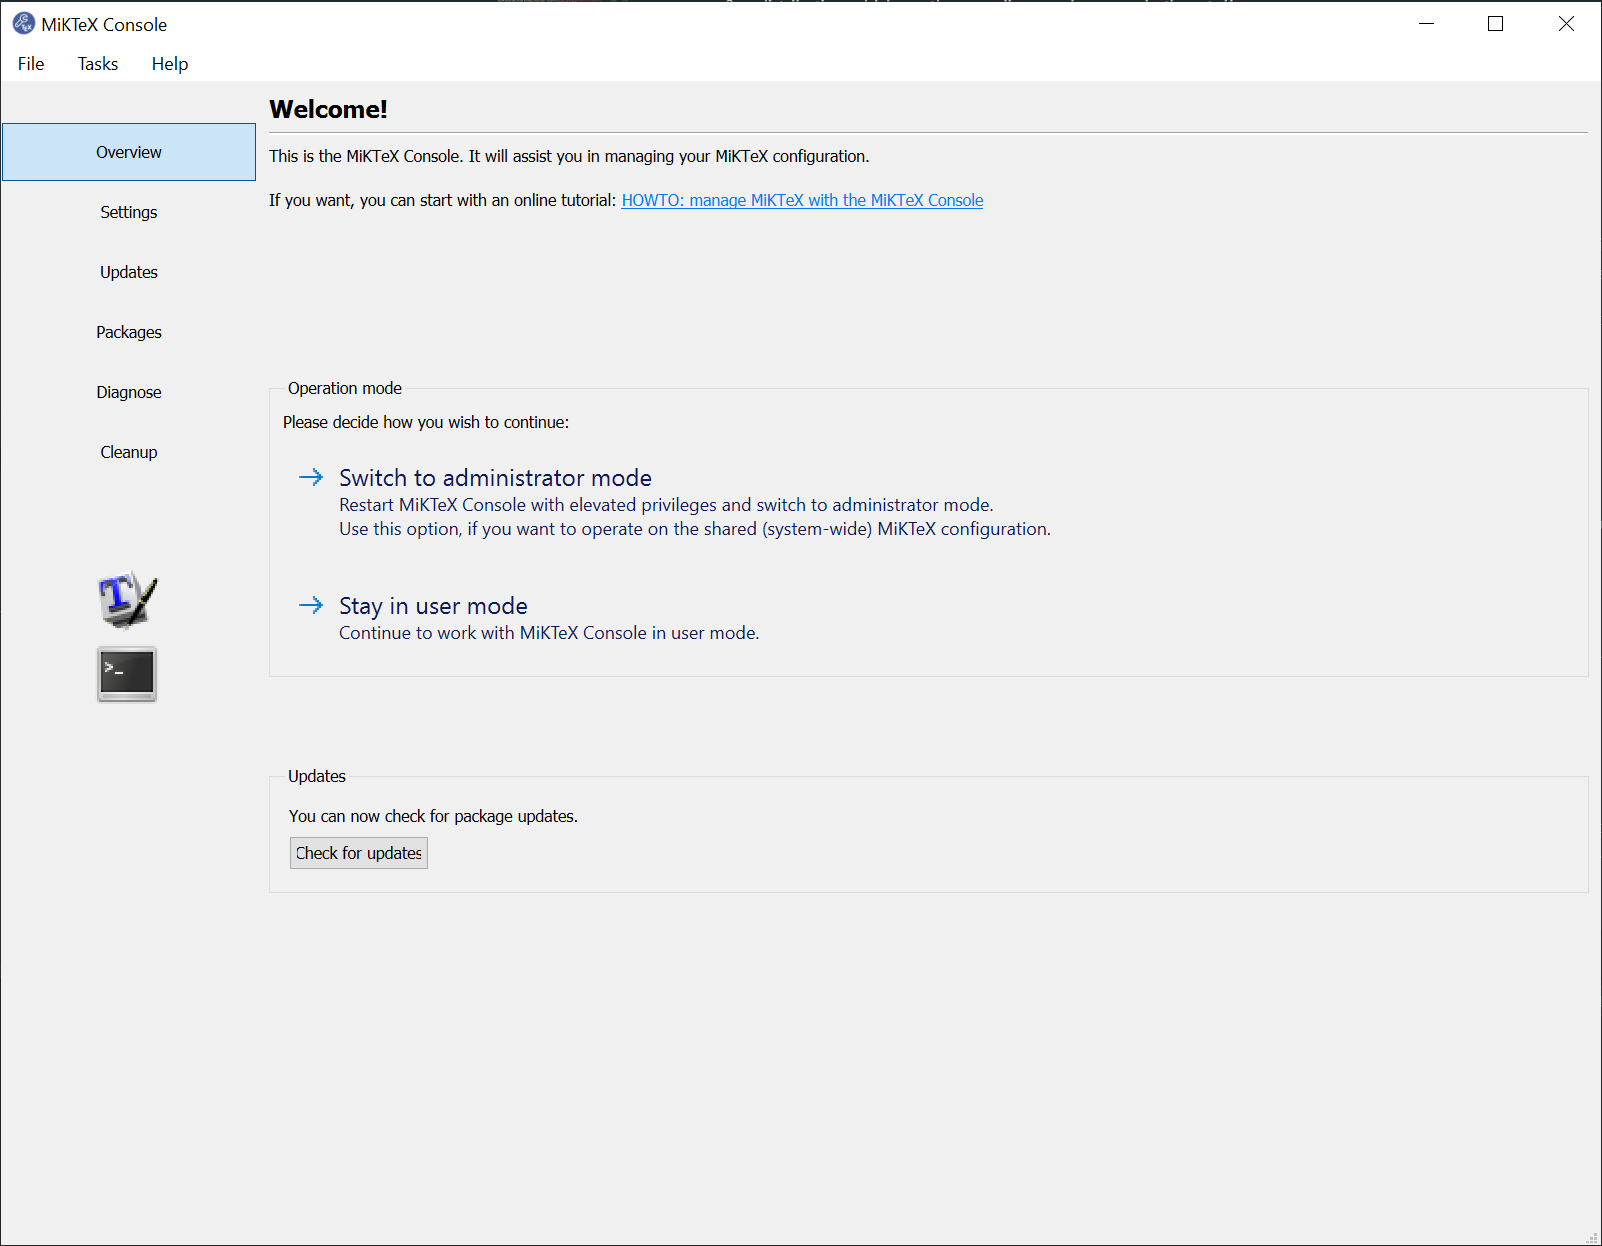
\includegraphics[width=0.5\textwidth]{miktex_gui}
        }%
    }
\end{figure}

\section{Glossaries}

\ctanpackage{glossaries-extra} is an absolute unit of a package.
For this document, it is used with its back\-/end \ctanpackage{bib2gls}.
This Java tool comes with installations of TeXLive and MiKTeX.
You should already have it.

In a format similar to normal bibliographies, all glossary entries are now managed
using \texttt{*.bib} files.
Each entry is processed by \ctanpackage{bib2gls} and put into an auxiliary file.
From it, it reads and inserts all contents when \verb|\gls| and its many siblings
are used.
The framework for all of that, also printing of the glossary and nomenclature,
is already taken care of for this document.

Traditionally, glossary packages are used for abbreviations.
However, using \ctanpackage{glossaries-extra} this can be kicked into top gear.
It is used for:
\begin{itemize}
    \item abbreviations,
    \item (physical) constants,
    \item symbols (greek, roman and all other),
    \item subscripts,
    \item the book index, consisting of names and the normal index.
\end{itemize}

In the case of symbols, this means the source now relies on \verb|\sym{<label>}|
commands.
For example, equations no longer read \verb|E = mc^{2}|, but instead
\begin{verbatim}
    \sym{energy} = \sym{mass}\sym{velocity}^{2}
\end{verbatim}
This initially unintuitive approach has several critical advantages:
\begin{enumerate}
    \item absolute \textbf{consistency} following the \abb{single_source_of_truth}
        principle:
        there is exactly \emph{one} place where the symbol itself is defined.
        All other usages are just \emph{references} to this central definition.
        If suddenly, the symbol for velocity has to change from \(c\) to \(v\)
        throughout the entire document, it can be done with ease.
        Replacing single letters like that using tools like \texttt{sed} would be a
        nightmare, if not impossible.

        There is also absolutely no danger that \emph{both} symbols occur (unless
        it is explicitly set up like that), with both referring to velocity,
        as can happen when returning to a document after abandoning it for many months
        or if multiple authors work on one document.
    \item following the \textbf{\abb{what_you_see_is_what_you_mean}} principle:
        this is \LaTeX{}'s big strength.
        In the source code, it no longer states what you \emph{want to see}, but
        instead \emph{what you mean}.
        When you write \verb|E = mc^2|, you are writing what you want to see:
        the letter \texttt{E} is somehow equal to the product of letter \texttt{m}
        times \texttt{c} squared.
        But the \emph{meaning} is that \emph{energy} equals \emph{mass} times
        \emph{velocity} squared.
        This can now be expressed directly in the source code.

        The \abb{what_you_see_is_what_you_mean} principle is at the core of \LaTeX{}
        and is what sets it apart.
        It is the reason you also do not say
        \begin{verbatim}
            {\Huge\textsf{\textbf{<Section Title>}}}
        \end{verbatim}
        but instead simply
        \begin{verbatim}
            \section{<Section Title>}
        \end{verbatim}
        In the first, it was stated what the author wants to \emph{see}, but only
        in the second one does it say what was \emph{meant}.
        It is painfully obvious why the latter approach is the correct one.
        This is a trap beginners unfortunately often fall into.
        Using \ctanpackage{glossaries-extra}, abstracted markup\-/commands can be
        taken to a whole next level, leveraging this core \LaTeX{} strength.
    \item \textbf{abolishing ambiguity}:
        especially when the source code is read by other people, or even worked on,
        \enquote{naked} symbols can become ambiguous.
        What American authors refer to with a capital \emph{P}, European authors
        interpret as \emph{power}, when really \emph{pressure} was meant.
        This is a non\-/issue if in the source it says \verb|\sym{pressure}|.
        For internationalization, authors would then only adjust their
        \emph{style-sheets} (in this case the \texttt{*.bib} files) and be done.
    \item arguably improving \textbf{readability}.
        The source code can almost be read like a normal sentence consisting of full
        words, albeit with braces and backslashes in the way.
    \item printing the \textbf{nomenclature} becomes trivial.
        A single command simply prints the \texttt{*.bib} file contents.
        Being an external Java tool, the customization, sorting and filtering
        capabilities of \ctanpackage{bib2gls} for printing those lists are likely
        more than will ever be needed.
    \item lastly, some more gimmicky features are enabled, like printing all
        page numbers of occurrences of a symbol.
        Alternatively, only the first occurrence can be printed.
\end{enumerate}

\section{MATLAB/Simulink icons}

For an older project, MATLAB/Simulink vector icons were created.
They are included here at the off chance that someone else might find a use for these.
\begin{itemize}
    \item \mtlbsmlkicon{matlab_object_box}
    \item \mtlbsmlkicon{matlab_struct}
    \item \mtlbsmlkicon{matlab_table}
    \item \mtlbsmlkicon{simulink_algebraic_constraint}
    \item \mtlbsmlkicon{simulink_base_workspace}
    \item \mtlbsmlkicon{simulink_configuration}
    \item \mtlbsmlkicon{simulink_data_dictionary}
    \item \mtlbsmlkicon{simulink_library_model}
    \item \mtlbsmlkicon{simulink_library}
    \item \mtlbsmlkicon{simulink_log_data}
    \item \mtlbsmlkicon{simulink_lut}
    \item \mtlbsmlkicon{simulink_model_workspace}
    \item \mtlbsmlkicon{simulink_model}
    \item \mtlbsmlkicon{simulink_referenced_model}
    \item \mtlbsmlkicon{simulink_step_block}
\end{itemize}

\begin{landscape}
    \section{Landscape}

    Pages in landscape format are rather straightforward to implement.
    Note that not only are these in landscape orientation; they are also recognized
    as such by supporting document viewers, rotating the page for you and keeping
    it legible.
\end{landscape}
